\chapter{\ploren{Rysunki, fotografie i podrysunki}{Figures, photographs and subfigures}}
\label{app:rysunki}

\begin{quote}
\itshape
\ploren
  {Ten załącznik zawiera przykłady instruktażowe przeznaczone do usunięcia lub zastąpienia materiałami autora. Wygenerowane obrazy służą wyłącznie do demonstracji składu i nie przedstawiają rzeczywistych wyników badań.}
  {This appendix contains instructional examples that should be removed or replaced with the author's own material. The generated images are provided solely to demonstrate document layout and do not represent actual experimental results.}
\end{quote}

\section{\ploren{Zasady przygotowania materiałów graficznych}{Guidelines for preparing graphical material}}

Zasady przedstawione w tej sekcji dotyczą wszystkich rysunków, fotografii, wykresów, schematów i diagramów umieszczanych w pracy. Kolejne załączniki rozwijają wymagania właściwe dla poszczególnych rodzajów grafiki.

Niezależnie od użytego programu i rodzaju materiału należy przestrzegać następujących zasad:

\begin{itemize}
  \item preferować format PDF lub SVG dla grafiki wektorowej, a PNG dla grafiki rastrowej; JPG stosować przede wszystkim do fotografii,
  \item zapewnić minimalną czytelność tekstu, symboli i linii po przeskalowaniu do rozmiaru użytego w pracy,
  \item opisać osie wykresów i podać jednostki przedstawianych wielkości,
  \item rozróżniać serie danych nie tylko kolorem, lecz także rodzajem linii, znacznikiem lub innym oznaczeniem,
  \item sprawdzić czytelność materiału po wydruku w skali szarości,
  \item przywołać i omówić każdy rysunek, wykres, schemat oraz diagram w tekście,
  \item podać źródło materiału pochodzącego z publikacji lub innego zewnętrznego źródła,
  \item przechowywać edytowalny plik źródłowy, dane oraz skrypt generujący wynik.
\end{itemize}

\subsection{\ploren{Format i rozdzielczość}{Format and resolution}}

Format JPG jest odpowiedni przede wszystkim dla fotografii i obrazów zawierających wiele płynnych przejść tonalnych. Zastosowana kompresja zmniejsza rozmiar pliku, ale może wprowadzać widoczne zniekształcenia, dlatego nie należy wielokrotnie zapisywać tego samego obrazu w tym formacie. Format PNG stosuje kompresję bezstratną i jest zalecany dla grafiki rastrowej, na przykład zrzutów ekranu, map cieplnych, prostych ilustracji oraz obrazów wymagających przezroczystości.

Schematy, diagramy i wykresy należy w miarę możliwości zapisywać jako grafikę wektorową PDF lub SVG. Ponieważ bezpośrednia obsługa SVG zależy od środowiska kompilacji, w tym szablonie najbezpieczniej wyeksportować lub przekonwertować taki plik do PDF. Jeżeli dostępny jest tylko JPG lub PNG, plik powinien mieć rozdzielczość wystarczającą do zachowania czytelności po umieszczeniu w docelowym rozmiarze. Sztuczne zwiększanie rozdzielczości nie przywraca utraconych szczegółów.

\subsection{\ploren{Czytelność i dostępność}{Readability and accessibility}}

Tekst, symbole i linie muszą pozostać czytelne po umieszczeniu obrazu w dokumencie. Należy stosować spójne kroje i wielkości pisma oraz unikać nadmiernej liczby kolorów. Znaczenie elementów nie powinno wynikać wyłącznie z koloru — serie danych warto dodatkowo rozróżniać rodzajem linii, znacznikiem lub opisem. Każdy materiał należy sprawdzić w docelowym rozmiarze oraz po wydruku w skali szarości.

Rysunek powinien przekazywać jedną czytelną informację i nie zawierać zbędnych elementów interfejsu programu. Osie, symbole, legendy i jednostki muszą być jednoznaczne. Tytułu wykresu nie trzeba powtarzać wewnątrz obrazu, jeżeli jego funkcję spełnia podpis utworzony w LaTeX.

\subsection{\ploren{Pliki źródłowe i powtarzalność}{Source files and reproducibility}}

Oprócz obrazu użytego w pracy należy zachować jego edytowalny plik źródłowy, dane oraz skrypt generujący, jeżeli istnieją. Eksporty umieszcza się w katalogu \texttt{figures}, a materiały źródłowe w podkatalogu \texttt{figures/source}. Pozwala to poprawić rysunek lub wygenerować go ponownie bez ręcznego odtwarzania ustawień.

\section{\ploren{Pojedynczy rysunek lub fotografia}{A single figure or photograph}}

Każdy rysunek powinien zostać zapowiedziany i omówiony w tekście. Na rysunku~\ref{fig:stanowisko-elektroniczne} przedstawiono przykładową wizualizację stanowiska elektronicznego. Plik JPG umieszczono w katalogu \texttt{figures} należącym do tego załącznika.

\begin{figure}[htbp]
  \centering
  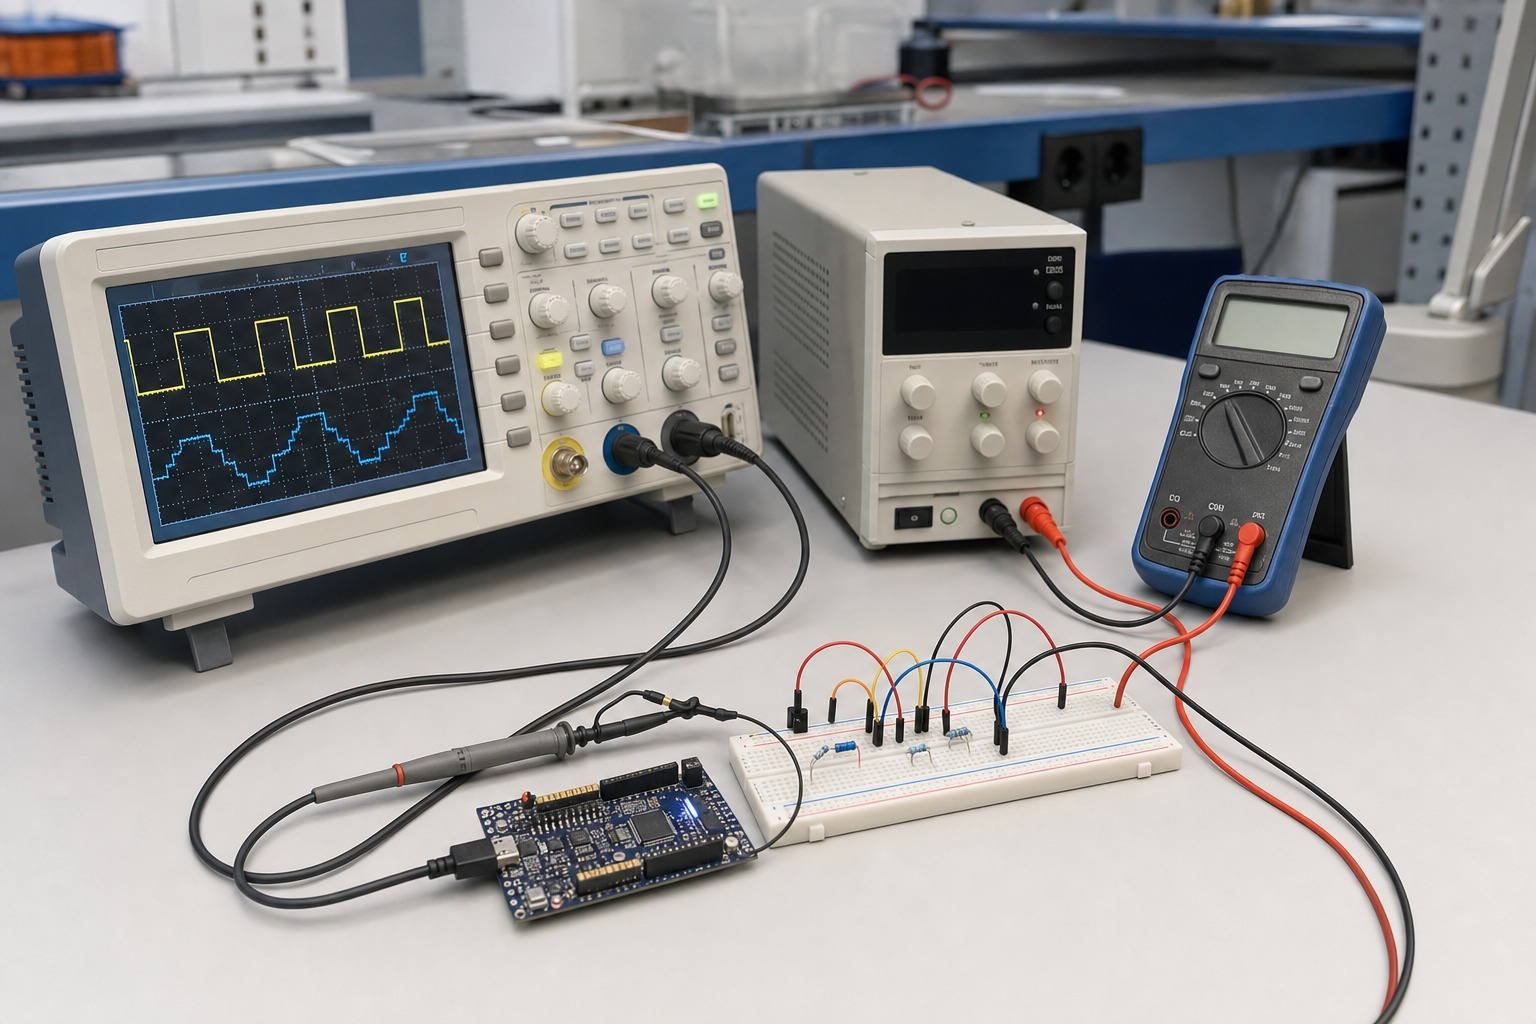
\includegraphics[width=0.88\textwidth]{chapters/10-zalacznik-c-rysunki/figures/stanowisko-elektroniczne.jpg}
  \caption{\ploren
    {Przykładowa wizualizacja stanowiska do badań układu elektronicznego (materiał wygenerowany na potrzeby szablonu)}
    {Example visualisation of an electronic circuit test bench (material generated for this template)}}
  \label{fig:stanowisko-elektroniczne}
\end{figure}

\begin{lstlisting}[caption={\ploren{Kod pojedynczego rysunku}{Code for a single figure}}]
Jak przedstawiono na rysunku~\ref{fig:stanowisko-elektroniczne}, ...

\begin{figure}[htbp]
  \centering
  \includegraphics[width=0.88\textwidth]{sciezka/do/obrazu.jpg}
  \caption{Opis zawartości rysunku}
  \label{fig:stanowisko-elektroniczne}
\end{figure}
\end{lstlisting}

Opcja \verb|width=0.88\textwidth| skaluje obraz względem szerokości obszaru tekstu i zapobiega jego wyjściu poza margines. Nie należy jednocześnie podawać szerokości i wysokości bez opcji zachowania proporcji, ponieważ może to zniekształcić obraz. Etykietę \verb|\label| umieszcza się po poleceniu \verb|\caption|.

\subsection{\ploren{Położenie obiektu i parametry obrazu}{Float placement and image options}}

Zapis \verb|[htbp]| przy środowisku \texttt{figure} określa dozwolone, preferowane miejsca umieszczenia obiektu pływającego. Kolejne litery oznaczają:

\begin{itemize}
  \item \texttt{h} (ang. \emph{here}) — możliwie blisko miejsca wystąpienia w kodzie,
  \item \texttt{t} (ang. \emph{top}) — u góry strony,
  \item \texttt{b} (ang. \emph{bottom}) — u dołu strony,
  \item \texttt{p} (ang. \emph{page}) — na osobnej stronie przeznaczonej na obiekty pływające.
\end{itemize}

LaTeX sprawdza wskazane możliwości i wybiera miejsce spełniające reguły składu. Zapis \verb|[htbp]| nie oznacza zatem bezwarunkowego umieszczenia rysunku dokładnie w miejscu wpisania kodu. Kolejność liter określa preferencje autora, ale ostateczna decyzja zależy także od dostępnego miejsca i liczby obiektów pływających.

Można użyć innych kombinacji, na przykład \verb|[tbp]|, \verb|[ht]| albo \verb|[p]|. Modyfikator \texttt{!}, na przykład w zapisie \verb|[!htbp]|, zezwala LaTeXowi na złagodzenie części wewnętrznych ograniczeń dotyczących rozmieszczania obiektów. Nie powinien być dodawany automatycznie do każdego rysunku. Specyfikator \texttt{H}, znany z pakietu \texttt{float}, wymusza położenie w konkretnym miejscu, ale nie jest standardowym znacznikiem środowiska \texttt{figure} i jego nadużywanie często pogarsza skład strony. Gdy rysunki nie powinny przechodzić do kolejnej części dokumentu, można zastosować polecenie \verb|\FloatBarrier|.

Opcje w nawiasach kwadratowych polecenia \verb|\includegraphics| sterują natomiast wyglądem samego obrazu. Najczęściej wykorzystuje się:

\begin{itemize}
  \item \verb|width=...| — szerokość obrazu,
  \item \verb|height=...| — wysokość obrazu,
  \item \verb|scale=...| — skalowanie względem rozmiaru naturalnego,
  \item \verb|keepaspectratio| — zachowanie proporcji przy jednoczesnym ograniczeniu szerokości i wysokości,
  \item \verb|angle=...| — obrót obrazu,
  \item \verb|trim=lewo dół prawo góra,clip| — przycięcie wskazanych krawędzi.
\end{itemize}

Przykładowo zapis:

\begin{lstlisting}[numbers=none]
\includegraphics[
  width=\textwidth,
  height=0.75\textheight,
  keepaspectratio
]{figures/obraz.png}
\end{lstlisting}

ogranicza obraz jednocześnie szerokością i wysokością strony bez zmiany jego proporcji. Pakiet \texttt{graphicx} oferuje również inne opcje; w pracy należy stosować tylko te, które rozwiązują konkretny problem i nie pogarszają czytelności materiału.

\section{\ploren{Podrysunki}{Subfigures}}

Podrysunki stosuje się, gdy kilka obrazów tworzy jedno logiczne porównanie i powinno mieć wspólny numer. Rysunek~\ref{fig:stanowiska-porownanie} zestawia dwa przykładowe stanowiska, natomiast rysunki~\ref{fig:stanowisko-automatyki} i~\ref{fig:stanowisko-wbudowane} pozwalają przywołać osobno część~(a) i~(b).

\begin{figure}[htbp]
  \centering
  \begin{subfigure}[t]{0.48\textwidth}
    \centering
    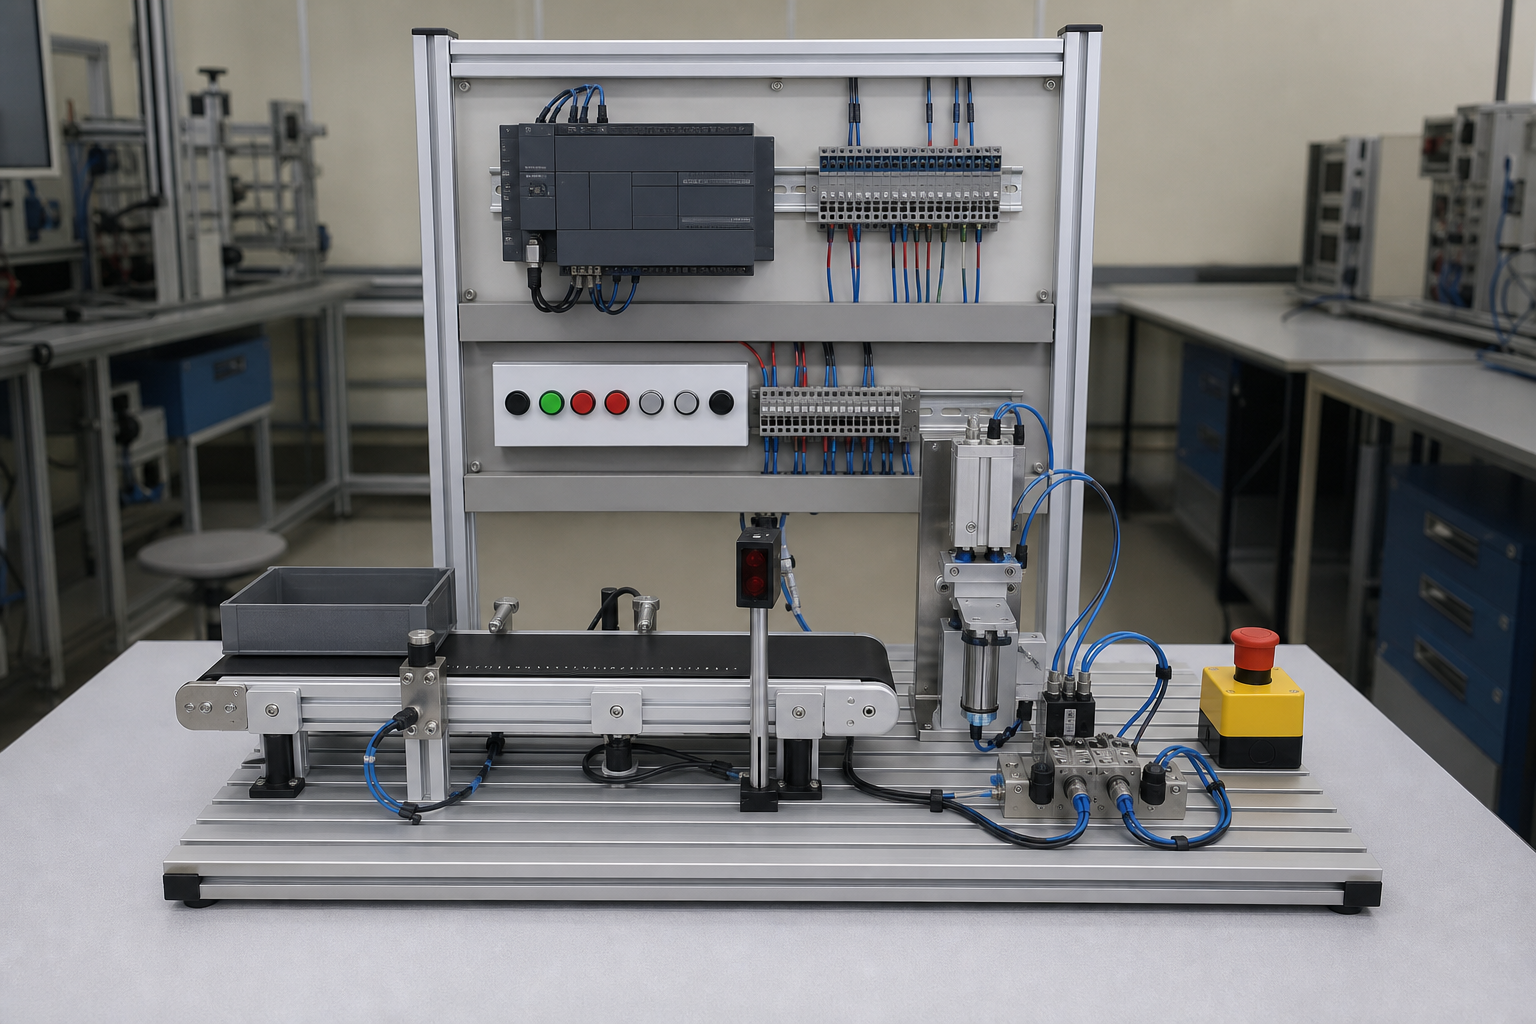
\includegraphics[width=\linewidth]{chapters/10-zalacznik-c-rysunki/figures/stanowisko-automatyki.png}
    \caption{\ploren{Stanowisko automatyki}{Automation training station}}
    \label{fig:stanowisko-automatyki}
  \end{subfigure}
  \hfill
  \begin{subfigure}[t]{0.48\textwidth}
    \centering
    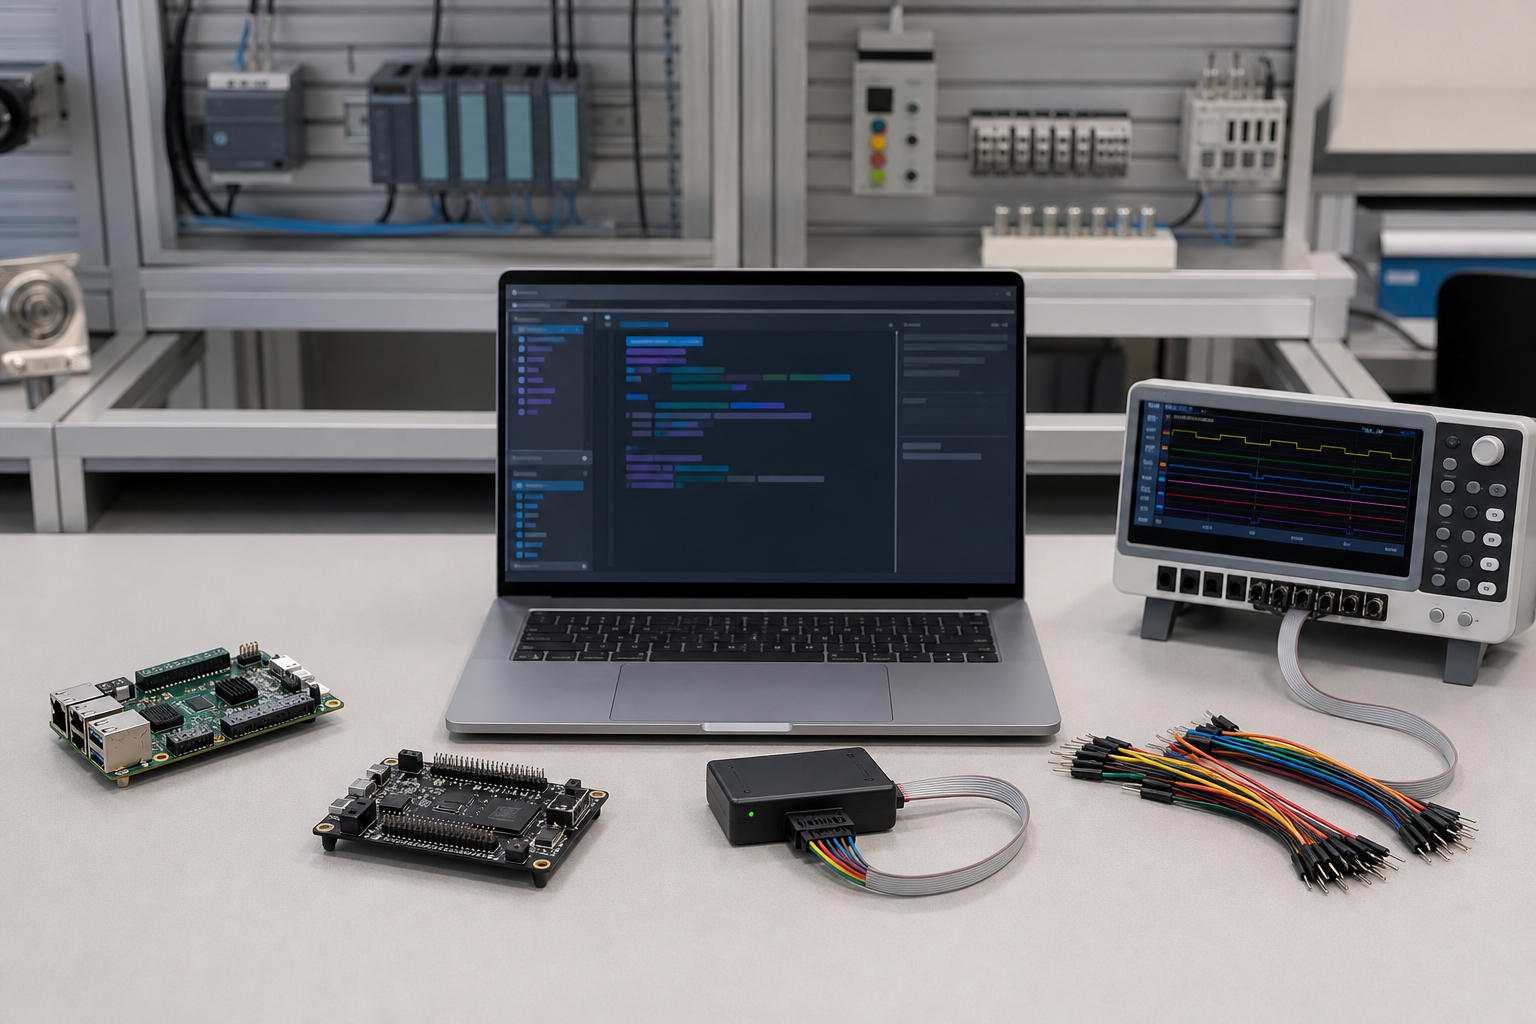
\includegraphics[width=\linewidth]{chapters/10-zalacznik-c-rysunki/figures/stanowisko-systemow-wbudowanych.png}
    \caption{\ploren{Stanowisko systemów wbudowanych}{Embedded systems workstation}}
    \label{fig:stanowisko-wbudowane}
  \end{subfigure}
  \caption{\ploren
    {Przykładowe stanowiska laboratoryjne (materiały wygenerowane na potrzeby szablonu)}
    {Example laboratory workstations (materials generated for this template)}}
  \label{fig:stanowiska-porownanie}
\end{figure}

\begin{lstlisting}[caption={\ploren{Kod dwóch podrysunków}{Code for two subfigures}}]
\begin{figure}[htbp]
  \centering
  \begin{subfigure}[t]{0.48\textwidth}
    \centering
    \includegraphics[width=\linewidth]{figures/obraz-a.png}
    \caption{Pierwszy wariant}
    \label{fig:wariant-a}
  \end{subfigure}
  \hfill
  \begin{subfigure}[t]{0.48\textwidth}
    \centering
    \includegraphics[width=\linewidth]{figures/obraz-b.png}
    \caption{Drugi wariant}
    \label{fig:wariant-b}
  \end{subfigure}
  \caption{Porównanie dwóch wariantów}
  \label{fig:porownanie-wariantow}
\end{figure}
\end{lstlisting}

Szerokości podrysunków powinny pozostawiać miejsce na odstęp pomiędzy nimi. Dla dwóch elementów zwykle sprawdza się wartość od \num{0.47} do \num{0.49} szerokości tekstu. Jeżeli obrazy stają się nieczytelne, lepiej umieścić je jeden pod drugim niż nadmiernie je zmniejszać.

\section{\ploren{Podpis, źródło i odwołanie}{Caption, source and cross-reference}}

Podpis powinien opisywać znaczenie rysunku, a nie tylko powtarzać nazwę przedstawionego obiektu. Dla materiału zaadaptowanego lub odtworzonego na podstawie publikacji należy podać cytowanie w podpisie i jasno określić zakres modyfikacji. Sam adres strony internetowej nie zastępuje kompletnego wpisu bibliograficznego.

Fotografia dokumentująca stanowisko lub wynik eksperymentu powinna przedstawiać rzeczywisty obiekt. Obrazu wygenerowanego, demonstracyjnego albo poglądowego nie wolno opisywać w sposób sugerujący, że jest dokumentacją przeprowadzonych badań. Informację o wykorzystaniu narzędzia generatywnego należy podać zgodnie z zasadami przyjętymi dla pracy.

Do rysunków należy odwoływać się przez etykiety. Pierwszy sposób wykorzystuje standardowe polecenie \verb|\ref| i pozostawia autorowi kontrolę nad formą gramatyczną nazwy:

\begin{center}
\verb|rysunek~\ref{fig:stanowisko-elektroniczne}|
\end{center}

W zdaniu można odpowiednio napisać:

\begin{center}
\verb|na rysunku~\ref{...}|
\qquad
\verb|zgodnie z rysunkiem~\ref{...}|
\end{center}

Polecenie \verb|\ref| wstawia wyłącznie numer.

Drugi sposób wykorzystuje pakiet \texttt{cleveref}, który automatycznie dodaje nazwę rodzaju elementu:

\begin{center}
\verb|\cref{fig:stanowisko-elektroniczne}|
\end{center}

Polecenie \verb|\cref| tworzy zapis „rysunek~\ref{fig:stanowisko-elektroniczne}”, natomiast \verb|\Cref| rozpoczyna nazwę wielką literą. Można również przekazać kilka etykiet w jednym poleceniu:

\begin{lstlisting}[numbers=none]
\cref{fig:stanowisko-automatyki,
      fig:stanowisko-wbudowane}
\end{lstlisting}

Nazwa, liczba mnoga i spójnik zostaną wtedy dobrane automatycznie.

Obydwa sposoby zachowują automatyczną numerację. Nie należy ręcznie wpisywać numerów ani używać określeń „rysunek powyżej” lub „rysunek poniżej”. W jednym dokumencie warto przyjąć jeden podstawowy sposób i stosować go konsekwentnie.

\section{\ploren{Najczęstsze błędy}{Common mistakes}}

Do najczęstszych problemów należą obrazy o zbyt małej rozdzielczości, tekst nieczytelny po przeskalowaniu, brak jednostek i legendy, zbyt długie podpisy, niepodanie źródła, brak odwołania w treści oraz stosowanie zrzutu ekranu zamiast eksportu właściwego rysunku. Należy również unikać umieszczania tytułu wewnątrz obrazu, jeżeli tę samą funkcję spełnia podpis LaTeX.
